\documentclass{article}
\AtBeginDocument{\RenewCommandCopy\qty\SI}
\usepackage{style}
\title{ECE355 Cheatsheet}
\author{Hanhee Lee}
\lhead{ECE355}
\rhead{Hanhee Lee}

\begin{document}
\maketitle

\tableofcontents

\listoffigures

\listoftables

\section{Tips}
\begin{intuition}
    \begin{itemize}
        \item May diverge from textbook, but only responsible for lecture content.
        \item Tutorials: Review of last week's topics and assigned problems. 
        \item Piazza for asking questions.
        \item ISM: Investigate topic of interest that uses signals or systems with 10 pages that are reference, explain concepts in your own way.
        \item Quiz every week except for term tests. 
        \item 30 minutes, appears Tuesday morning and ends Tuesday night. 
        \item Easier than usual questions that tests understanding. 
        \item Open book with MC, numerical answer. 
    \end{itemize}
\end{intuition}

\section{Mathematical Review}
\subsection{Sets}
\begin{definition}
    An unordered collection of objects (i.e. elements or members)
    \begin{itemize}
        \item A set \emph{contains} its elements or elements of a set are \emph{contained in} that set.
    \end{itemize}
\end{definition}

    \subsubsection{Set notation}
    \begin{terminology}
        \begin{itemize}
            \item $\ldots$ mean "and so on"
            \item $:$ mean "such that"
            \item $\in$ mean "contained"
            \item $\notin$ mean "not contained"
            \item $\emptyset$ mean "empty set (i.e. a set contains no elements")
            \item $A\subseteq B$ mean "Only if every element of $A$ is also an element of $B$"
            \item $B\supseteq A$ mean "B is a superset of A to mean A is a subset of B" 
            \item Normally, elements of a set are listed just once.
        \end{itemize}
    \end{terminology}

\begin{example}

    \textbf{Sets:}
    \begin{itemize}
        \item $E = \{0,2,4,6,8\}$, where $2\in E$ and $1 \notin E$
        \item $\mathbb{Z} = \{\ldots,-2,-1,0,1,2,\ldots\}$
        \item $P=\{0,1,...,255\}$
        \item $O = \{x \in \mathbb{Z}: \; x=2k+1 \text{ for some } k \in \mathbb{Z}\}$
        \item $\{\emptyset,\{\emptyset\}\}$ (i.e. A set that has other sets as elements).
    \end{itemize}
    \vspace{1em}

    \textbf{Subset:}
    \begin{itemize}
        \item $E \subseteq \mathbb{Z}$
    \end{itemize}
\end{example}

\begin{theorem}
    $A = B$ means $A \subseteq B$ and $B \subseteq A$.
    \begin{itemize}
        \item \textbf{Note:} Have to prove in both directions.
    \end{itemize}
\end{theorem}

\begin{example}
    $\{1,2,3\}=\{3,2,1,1,2\}$
\end{example}

    \subsubsection{Important sets}
    \begin{definition}
        \begin{enumerate}
            \item \textbf{Natural:} \( \mathbb{N} = \{0, 1, 2, 3, \dots \} \): 
            \item \textbf{Integers:} \( \mathbb{Z} = \{ \dots, -2, -1, 0, 1, 2, \dots \} \): 
            \item \textbf{Rational:} \( \mathbb{Q} = \left\{ \frac{a}{b} : a, b \in \mathbb{Z}, b \neq 0 \right\} \): 
            \item \textbf{Real:} \( \mathbb{R} \): 
            \item \textbf{Complex:} \( \mathbb{C} = \{ a + bj : a, b \in \mathbb{R} \} \)
            \begin{itemize}
                \item \( j \): imaginary unit, where \( j^2 = -1 \) and \( j = \sqrt{-1} \)
            \end{itemize}
        \end{enumerate}  
        \begin{itemize}
            \item \textbf{Note:} $\mathbb{N} \subseteq \mathbb{Z} \subseteq \mathbb{Q} \subseteq \mathbb{R} \subseteq \mathbb{C} $
        \end{itemize}      
    \end{definition}

\subsection{Ordered n-tuples}
\begin{definition}
    An ordered collection of \( n \) elements, where \( n \) is a positive integer, denoted as \( (a_1, a_2, \dots, a_n) \), where \( a_1 \) is the first element, and so on, up to \( a_n \).
\end{definition}
    
    \subsubsection{How are two tuples equal?}
    \begin{definition}
        Unlike sets, both the order of elements and the repetition of values are significant. Therefore, two ordered \( n \)-tuples are considered equal (i.e. $(a_1, a_2, \dots, a_n) = (b_1, b_2, \dots, b_n)$) iff:

        \[
        a_1 = b_1, a_2 = b_2, \dots, a_n = b_n.
        \]
    \end{definition}

    \subsubsection{Cartesian product}
    \begin{definition}
        \textbf{Two sets:}
        The \textit{Cartesian product} of two sets \( A \) and \( B \) (in that order), denoted as \( A \times B \), is the set of all \textit{ordered pairs} or \textit{ordered 2-tuples} \( (a, b) \) where \( a \in A \) and \( b \in B \). Thus

        \begin{equation}
            A \times B = \{ (a, b) : a \in A, b \in B \}.    
        \end{equation}
        \begin{itemize}
            \item \textbf{General:} $B \times A \neq A \times B$
            \item \textbf{2-fold Cartesian product:} $A \times A$ is denoted as $A^2$
        \end{itemize}
        \vspace{1em}

        \textbf{More than two sets:}
        The Cartesian product of sets \( A_1, A_2, \dots, A_n \), denoted as \( A_1 \times A_2 \times \cdots \times A_n \), is the set of ordered \( n \)-tuples \( (a_1, a_2, \dots, a_n) \), where \( a_1 \in A_1, a_2 \in A_2, \dots, a_n \in A_n \). Thus

        \begin{equation}
            A_1 \times A_2 \times \cdots \times A_n = \{(a_1, a_2, \dots, a_n) : a_1 \in A_1, a_2 \in A_2, \dots, a_n \in A_n\}.
        \end{equation}
        \begin{itemize}
            \item \textbf{n-fold Cartesian product:} $A\times A\times \cdots \times A$ is denoted as $A^n$
        \end{itemize}

    \end{definition}

\subsection{Functions}
\begin{definition}
    A function \( f: A \to B \) from a set \( A \) (the domain of \( f \)) to a set \( B \) (the codomain of \( f \)) assigns to each element \( a \in A \) exactly one element \( b \in B \), usually denoted as \( b = f(a) \).
\end{definition}

    \subsubsection{Range/Image}
    \begin{definition}
        \textbf{The range or image} of \( f \) is the subset of the codomain $B$ given as 
        \[
        \text{Im}_f(A) = \{ b \in B: \exists a \in A(f(a) = b) \}.
        \]
        \begin{itemize}
            \item \textbf{English:} Set of values "hit" by $f$ as its argument ranges over the set $A$.
        \end{itemize}
    \end{definition}

    \subsubsection{Inverse Image}
    \begin{definition}
        \textbf{The inverse image or pre-image} of any element \( b \in B \) under the mapping by \( f \) is the set 
        \[
        f^{-1}(b) = \{ a \in A : f(a) = b \}.
        \]
        \begin{itemize}
            \item \textbf{English:} Set of elements of the domain that map to $b$ under transformation by $f$.
            \item \textbf{Key:} If $b$ is an element of the codomain that is not in the range of $f$, then $f^{-1} (b) = \emptyset$
        \end{itemize}
    \end{definition}

\begin{example}
    \begin{itemize}
        \item Domain of \( g \): \( A = \{ 1, 2, 3, 4 \} \)
        \item Codomain of \( g \): \( B = \{ w, x, y, z \} \)
        \item Image of \( A \): \( \text{Im}_g(A) = \{ w, x, z \} \subseteq B \)
        \item Inverse Image
        \[
        g^{-1}(w) = \{ 1 \}
        \]
        \[
        g^{-1}(x) = \{ 2, 4 \}
        \]
        \[
        g^{-1}(y) = \emptyset
        \]
        \[
        g^{-1}(z) = \{ 3 \}
        \]
    \end{itemize}
    
    % Mapping Diagram
    \begin{center}
    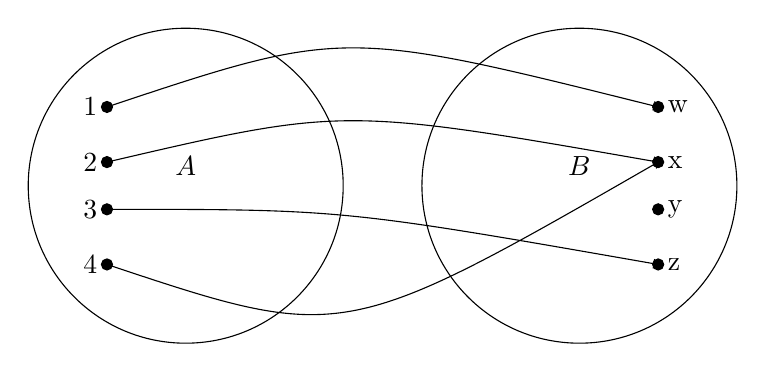
\begin{tikzpicture}
        % Sets A and B
        \draw (0, 0) circle (2cm) node[anchor=south] {$A$};
        \draw (5, 0) circle (2cm) node[anchor=south] {$B$};
    
        % Elements in A
        \filldraw[black] (-1, 1) circle (2pt) node[anchor=east] {1};
        \filldraw[black] (-1, 0.3) circle (2pt) node[anchor=east] {2};
        \filldraw[black] (-1, -0.3) circle (2pt) node[anchor=east] {3};
        \filldraw[black] (-1, -1) circle (2pt) node[anchor=east] {4};
    
        % Elements in B
        \filldraw[black] (6, 1) circle (2pt) node[anchor=west] {w};
        \filldraw[black] (6, 0.3) circle (2pt) node[anchor=west] {x};
        \filldraw[black] (6, -0.3) circle (2pt) node[anchor=west] {y};
        \filldraw[black] (6, -1) circle (2pt) node[anchor=west] {z};
    
        % Arrows for mappings
        \draw[->] (-1, 1) .. controls (2, 2) .. (6, 1);  % 1 -> w
        \draw[->] (-1, 0.3) .. controls (2, 1) .. (6, 0.3);  % 2 -> x
        \draw[->] (-1, -0.3) .. controls (2, -0.3) .. (6, -1);  % 3 -> z
        \draw[->] (-1, -1) .. controls (2, -2) .. (6, 0.3);  % 4 -> x
    \end{tikzpicture}
    \end{center}    
\end{example}

\subsection{Classes of functions}
    \subsubsection{Injective}
    \begin{definition}
        A function \( f: A \to B \) is called injective (or an injection or one-to-one) if $\forall a_1 \forall a_2$
        \[
        a_1 \neq a_2 \rightarrow f(a_1) \neq f(a_2).
        \]
        \[
        (f(a_1) = f(a_2) \rightarrow a_1 = a_2)
        \]

        \begin{itemize}
            \item \textbf{English:} Maps distinct elemetns of the domain to distinct elements of the codomain.
        \end{itemize}
        \customFigure[0.25]{00_Images/Injective.png}{Injective function.}
    \end{definition}

    \begin{process}
        Show a function is injective:
        \begin{enumerate}
            \item Set $f(x_1) = f(x_2)$
            \item Prove $x_1 = x_2$ from step 1. 
        \end{enumerate}
        \vspace{1em}

        Show a function is not injective:
        \begin{enumerate}
            \item Find a counterexample where $f(a_1) = f(a_2)$.
        \end{enumerate}
    \end{process}

    \subsubsection{Surjective}
    \begin{definition}
        A function \( f: A \to B \) is called surjective (or a surjection or onto) if 
        \[
        \forall b (f^{-1}(b) \neq \emptyset), \quad \text{or} \quad \forall b \exists a (f(a) = b),
        \]
        \begin{itemize}
            \item \textbf{English:} Every element in the codomain has a mapping back to the domain.
        \end{itemize}

        \customFigure[0.25]{00_Images/Surjective.png}{Surjective function.}
    \end{definition}

    \begin{process}
        Show a function is surjective:
        \begin{enumerate}
            \item Find the inverse of $f(x)=y$ by writing $x$ in terms of $y$ denoted $f^{-1}$
            \item See if the inverse satisfies the codomain, and there is no empty set.
        \end{enumerate}
        \vspace{1em}

        Show a function is not surjective:
        \begin{enumerate}
            \item Find a counterexample, where you get the empty set for $b\in B$
        \end{enumerate}
    \end{process}

    \begin{warning}
        Any nonsurjective function is a surjective function obtained from the original function by having the codomain match the range.
    \end{warning}

    \subsubsection{Bijective}
    \begin{definition}
        A function \( f: A \to B \) that is both injective and surjective is called bijective (or a bijection or a one-to-one correspondence).
        \begin{itemize}
            \item \textbf{Correspondence:} Inverse exists
        \end{itemize}
        \customFigure[0.25]{00_Images/Bijective.png}{Bijective function.}
    \end{definition}

\subsection{Composition of g with f}
\begin{definition}
    If \( f: A \to B \) and \( g: B \to C \), then \( g \circ f: A \to C \) s.t. $a \rightarrow g(f(a))$ (i.e. first apply $f$, then apply $g$)
    
    \customFigure[0.5]{00_Images/Composition.png}{Composition example}
    \begin{itemize}
        \item \textbf{Order is important:} $ f(g(a)) \neq g(f(a)) $
    \end{itemize}
\end{definition}

\subsection{Identity map}
\begin{definition}
    \[
    \text{id}_A: A \to A \quad \text{id}(a) = a \; \forall a \in A
    \]
\end{definition}

\subsection{Bijective property}
\begin{definition}
    Let \( f: A \to B \), then iff \( f \text{ is bijective, } \exists \text{ a function } f^{-1}: B \to A \text{ s.t. } f^{-1} \circ f = \text{id}_A \text{ and } f \circ f^{-1} = \text{id}_B \).
    \customFigure[0.5]{00_Images/Bijective_Property.png}{Illustration of bijective function}
\end{definition}

\subsection{Set of all functions with domain and codomain}
\begin{definition}
    The set of all fcns with domain $A$ and codomain $B$ is itself a set denoted $B^A$.
\end{definition}

\begin{example}
    % Example of the set of all functions from A to B
    If \( A = \{1, 2\} \) and \( B = \{x, y, z\} \), then \( B^A \) has \( 3^2 = 9 \) elements (i.e., \( B^A \)).

    \[
    f = \left( \begin{array}{c c}
    1 & 2 \\
    f(1) & f(2) \\
    \end{array} \right)
    \]

    The set \( B^A \) is:

    \[
    B^A = \left\{
    \left( \begin{array}{c c}
    1 & 2 \\
    x & x \\
    \end{array} \right),
    \left( \begin{array}{c c}
    1 & 2 \\
    x & y \\
    \end{array} \right),
    \left( \begin{array}{c c}
    1 & 2 \\
    x & z \\
    \end{array} \right),
    \left( \begin{array}{c c}
    1 & 2 \\
    y & x \\
    \end{array} \right),
    \left( \begin{array}{c c}
    1 & 2 \\
    y & y \\
    \end{array} \right),
    \left( \begin{array}{c c}
    1 & 2 \\
    y & z \\
    \end{array} \right),
    \left( \begin{array}{c c}
    1 & 2 \\
    z & x \\
    \end{array} \right),
    \left( \begin{array}{c c}
    1 & 2 \\
    z & y \\
    \end{array} \right),
    \left( \begin{array}{c c}
    1 & 2 \\
    z & z \\
    \end{array} \right)
    \right\}
    \]
\end{example}

\subsection{Complex math}
    \subsubsection{Complex number basics}
    \begin{definition}
    \begin{itemize}
        \item \( z = a + bj \), where \( a, b \in \mathbb{R} \)
        \begin{itemize}
            \item \( \text{Re}(z) = a \)
            \item \( \text{Im}(z) = b \)
        \end{itemize}
        
        \item \textbf{Complex conjugate:} If \( z = a + bj \), then \( z^* = a - bj \).
        
        \item \textbf{Magnitude:} \( |z| = \sqrt{z \cdot z^*} = \sqrt{a^2 + b^2} \).
    \end{itemize}

        % Complex plane diagram
        \begin{center}
        \begin{tikzpicture}
            \draw[->] (-0.5, 0) -- (3, 0) node[anchor=north] {$Re$};
            \draw[->] (0, -0.5) -- (0, 3) node[anchor=east] {$Im$};
            \filldraw[black] (2, 2) circle (2pt) node[anchor=south west] {$(a, b)$};
            \draw[->] (0, 0) -- (2, 2);
            \node at (2.3, -0.3) {$a$};
            \node at (-0.3, 2.3) {$b$};
        \end{tikzpicture}
        \end{center}

    \end{definition}

    \begin{example} 
        Expand the following function:
        \begin{align*}
            (a + bj)(c + dj) &= ac + (bc + ad)j + bdj^2 \\
            &= ac + (bc + ad)j - bd \quad \text{since} \, j^2 = -1.
        \end{align*}
    \end{example}

    \subsubsection{Complex exponential function}
    \begin{definition}
        % Exponential function definition
        \begin{equation}
            \exp: \mathbb{C} \to \mathbb{C} \text{ via } \exp(z) = 1 + z + \frac{z^2}{2!} + \frac{z^3}{3!} + \cdots = \sum_{k=0}^{\infty} \frac{z^k}{k!}    
        \end{equation}
        \begin{itemize}
            \item \textbf{Entire function:} Convergent no matter the values of z.
        \end{itemize}
        
        Let \( \theta \in \mathbb{R} \), the expansion of \( \exp(j\theta) \) is:
        \begin{equation}
            \exp(j\theta) = \cos \theta + j \sin \theta 
        \end{equation}
    \end{definition}

    \subsubsection{Complex plane with radius r}
    \begin{intuition}
        \customFigure[0.5]{00_Images/Complex_Plane_General.png}{Complex plane in general with radius r.}

        \begin{itemize}
            \item \textbf{Bounds:} $r \geq 0$ and $-\pi < \theta \leq \pi$
            \item \textbf{Polar:} Multiplication
            \item \textbf{Rectangular:} Additive
        \end{itemize}
    \end{intuition}

    \subsubsection{Complex conjugate}
    \begin{definition}
        \begin{equation}
            z^* = re^{-j\theta}
        \end{equation}
    \end{definition}

    \subsubsection{Converting between polar and rectangular form}
    \begin{process}

        \textbf{Polar to rectangular:} $e^{j\theta}$
        \begin{enumerate}
            \item Find $r$ and $\theta$ from $re^{j\theta}$
            \item Write in rectangular form: $z=rcos\theta + jrsin\theta$
        \end{enumerate}

        \textbf{Rectangular to polar:} $a+bj$
        \begin{enumerate}
            \item Find $r$ using Pythagorean theorem: $r = \sqrt{a^2 + b^2}$
            \item Find $\theta$ using trigonometry: $\theta = \text{tan}^{-1} \left(\frac{b}{a}\right)$, where $b$ is the opposite and $a$ is adjacent.
            \item Write in polar form: $z=re^{j\theta}$
        \end{enumerate}
        \begin{itemize}
            \item \textbf{Note:} Both forms can be found intuitively through a drawing of the complex plane. 
        \end{itemize}
    \end{process}

\subsection{Propositional logic}
    \subsubsection{Proposition}
    \begin{definition}
        A declarative statement that can be either \emph{true} or \emph{false}, denoted by a symbol (e.g. p or q).
    \end{definition}

    \subsubsection{Compound proposition}
    \begin{definition}
        Formed from existing propositions via negation and logical connectives.
    \end{definition}

    \subsubsection{Logical negation (logical not)}
    \begin{definition}
        An operation that takes a proposition $p$ to another proposition "not p", denoted $\neg p$ or $~p$.
        \customFigure[0.20]{00_Images/Truth_Table.png}{Truth table for negation.}
    \end{definition}
    
    \begin{example}
        What is the truth value of the double negation? 

        It is not the case that it is not the case that p is the same as that of p. 
        \begin{itemize}
            \item i.e. $\neg \neg p$ and $p$ to be \emph{logically equivalent}.
        \end{itemize}
    \end{example}

    \subsubsection{Logical conjunction (logical AND)}
    \begin{definition}
        Two propositions $p$ and $q$ can be connected with a logical conjunction, denoted $\land$. 
        \customFigure[0.25]{00_Images/And.png}{Truth table of AND, where truth value T only when $p$ and $q$ are truth.}
    \end{definition}
    
    \subsubsection{Logical disjunction (logical OR)}
    \begin{definition}
        Two propositions $p$ and $q$ can be connected with a logical disjunction, denoted $\lor$.  
        \customFigure[0.25]{00_Images/Or.png}{Truth table of OR, where truth value F only when both $p$ and $q$ are F and truth value T when either of $p$ or $q$ or both are true.}
    \end{definition}

    \subsubsection{De Morgan's Laws}
    \begin{definition}
        \begin{equation}
            \neg (p \land q) \equiv (\neg p) \lor (\neg q) \quad \text{and} \quad \neg (p \lor q) \equiv (\neg p) \land (\neg q)
        \end{equation}
    \end{definition}

    \subsubsection{Logical implication}
    \begin{definition}
        Two propositions \( p \) and \( q \) can be connected with a logical \textit{implication} denoted \( \to \) or “implies,” to form the logical proposition \( p \to q \).
        \begin{itemize}
            \item \textbf{Antecedent:} \( p \).
            \item \textbf{Consequent:} \( q \). 
            \item \textbf{English:} The proposition \( p \to q \) can be translated into English as “if \( p \) then \( q \),” or “\( q \) if \( p \).” 
            \item \textbf{Logically equivalent:} $p \to q$ and $\neg p \lor q$
        \end{itemize}
        \customFigure[0.25]{00_Images/Implication.png}{Truth table of logical implication, where truth value F only when $p$ is true and $q$ is false}
    \end{definition}

    \begin{warning} The following all mean the same thing:
        \begin{itemize}
            \item $p \rightarrow q$
            \item $p$ implies $q$
            \item if $p$, then $q$
            \item $q$ if $p$
            \item $p$ is a sufficient condition for $q$
            \item $p$ only if $q$ (i.e. $p \rightarrow q \equiv \neg q \rightarrow \neg p$ i.e. implication is logically equivalent to its contrapositive)
            \item $q$ is a necessary condition for $p$
        \end{itemize}        
    \end{warning}

    \subsubsection{Converse, inverse, contrapositive}
    \begin{definition}
        Let \( p \to q \) be a proposition. The following are the related forms of this proposition:

        \begin{itemize}
            \item The \textit{converse} of \( p \to q \) is the proposition \( q \to p \).
            \item The \textit{inverse} of \( p \to q \) is the proposition \( \neg p \to \neg q \).
            \item The \textit{contrapositive} of \( p \to q \) is the proposition \( \neg q \to \neg p \).
        \end{itemize}

        \customFigure[0.5]{00_Images/Converse.png}{Truth table}
    \end{definition}

    \begin{warning}
        The converse of an implication is \emph{not} logically equivalent to the implication.
    \end{warning}

    \subsubsection{Biconditional}
    \begin{definition}
        Two propositions $p$ and $q$ can be connected with a logical \textit{biconditional}, denoted $\leftrightarrow$ or "iff' to form the logical proposition $p \leftrightarrow q$.
        \customFigure[0.25]{00_Images/IFF.png}{Truth table of biconditional, where having truth value "true" whenever $p$ and $q$ have the same truth value, and "false" whenever $p$ and $q$ have different truth values.}
        \begin{itemize}
            \item \textbf{Logically equivalent:} The biconditional is logically equivalent to the conjunction $(p \rightarrow q) \land (q \rightarrow p)$ of an implication and its converse. 
        \end{itemize}
    \end{definition}

    \subsubsection{Rules of inference}
    Logic is used to deduce truth of certain propositions from the truth of other propositions.
    \begin{definition}
        \begin{enumerate}
            \item \textbf{Modus ponens (MP):}
                % Modus Ponens (MP)
                \[
                \frac{p \rightarrow q, \ p}{\therefore q}
                \]
                (If \(p \rightarrow q\) and \(p\) are both true, then \(q\).)
    
            \item \textbf{Modus tollens (MT):}
               % Modus Tollens (MT)
                \[
                \frac{p \rightarrow q, \ \neg q}{\therefore \neg p}
                \]
                (If \(p \rightarrow q\) and \(\neg q\) are both true, then \(\neg p\).)
            \item \textbf{Modus tellendo ponens (MTP):}
                % Modus Tollendo Ponens (MTP)
                \[
                \frac{p \lor q, \ \neg p}{\therefore q}
                \]
                (If \(p \lor q\) and \(\neg p\) are both true, then \(q\).)
            \item \textbf{Modus ponendo tollens (MPT):}
                % Modus Ponendo Tollens (MPT)
                \[
                \frac{\neg(p \land q), \ p}{\therefore \neg q}
                \]
                (If \(\neg(p \land q)\) and \(p\) are both true, then \(\neg q\).)
        \end{enumerate}
    \end{definition}

\subsection{Predicate logic}
\begin{definition}
    Defined via \emph{predicates}, which are prototypes for propositions involving \emph{predicate variables} (i.e. placeholder variables), each associated with a specific set (i.e. \emph{domain of discourse} for that variable)
    \begin{itemize}
        \item \textbf{Key:} When specific values from the domains of discourse are substituted for each of the predicate variables in a predicate, a specific proposition with a truth value is obtained.
    \end{itemize}
\end{definition}
    
    \subsubsection{Quantifiers}
    \begin{definition}
       
        \begin{enumerate}
            \item \textbf{Universal quantifier}, denoted $\forall$. When applied to a predicate $P(x)$, it asserts that the proposition $P(x)$ is true for every $x$ in the domain of discourse. Formally, it is written as $\forall x (P(x))$.
            \begin{itemize}
                \item Effects the conjunction (AND)
            \end{itemize}
            \item \textbf{Existential quantifier}, denoted $\exists$. When applied to a predicate $P(x)$, it asserts that the proposition $P(x)$ is true for at least one $x$ in the domain of discourse. Formally, it is written as $\exists x (P(x))$.
            \begin{itemize}
                \item Effects the disjunction (OR)
                \item $\exists x\in A(P(x)) \equiv \exists x (x\in A \land P(x)) $
            \end{itemize}
        \end{enumerate}
    \end{definition}

    \subsubsection{De Morgan's Law}
    \begin{definition}
        \begin{equation}
            \neg(\forall x (P(x))) \equiv \exists x (\neg P(x))    
        \end{equation}
        \begin{itemize}
            \item \textbf{English:} Failure of P to hold universally is equivalent to the existence of at least one element in the domain of discourse for which P fails to hold. 
        \end{itemize}
        \begin{equation}
            \neg(\exists x (P(x))) \equiv \forall x (\neg P(x))
        \end{equation}
        \begin{itemize}
            \item \textbf{English:} Failure of the existence of an element for which P holds is equivalent to P failing to hold for all elements in the domain of discourse
        \end{itemize}
    \end{definition}


\newpage

\section*{Signals and General Systems}
\section{Continuous and discrete-time signals (Ch. 1.1)}
\subsection{Signal energy and power}
    \subsubsection{Total energy}
    \begin{definition}
        
        \textbf{Continuous:} Total energy from $t_1 \leq t \leq t_2$ is 
        \begin{equation}
            E_{[t_1,t_2]} = \int_{t_1}^{t_2} \abs{x(t)}^2 dt
        \end{equation}
        \begin{itemize}
            \item $x(t)$: Continuous-time signal
            \item $\abs{x}$: Magnitude of the number
        \end{itemize}

        \textbf{Discrete:} Total energy from $n_1 \leq n \leq n_2$ is
        \begin{equation}
            E_{[t_1,t_2]} = \sum_{n=n_1}^{n_2} \abs{x[n]}^2
        \end{equation}
        \begin{itemize}
            \item $x[t]$: Discrete-time signal
        \end{itemize}
    \end{definition}

    \subsubsection{Average power}
    \begin{definition}

        \textbf{Continuous:} Average power from $t_1 \leq t \leq t_2$ is 
        \begin{equation}
            P_{[t_1,t_2]} = \frac{E_{[t_1,t_2]}}{t_2 - t_1} 
        \end{equation}

        \textbf{Discrete:} Average power from $n_1 \leq n \leq n_2$ is
        \begin{equation}
            P_{[t_1,t_2]} = \frac{E_{[t_1,t_2]}}{n_2 - n_1 + 1} 
        \end{equation}
    \end{definition}

    \subsubsection{Total energy over infinite time interval}
    \begin{definition}

        \textbf{Continuous:}
        \begin{equation}
            E_{\infty} \triangleq \lim_{T \to \infty} \int_{-T}^{T} |x(t)|^2 \, dt = \int_{-\infty}^{\infty} |x(t)|^2 \, dt
        \end{equation}

        \textbf{Discrete:}
        \begin{equation}
            E_{\infty} \triangleq \lim_{N \to \infty} \sum_{n=-N}^{+N} |x[n]|^2 = \sum_{n=-\infty}^{\infty} |x[n]|^2
        \end{equation}
    \end{definition}

    \subsubsection{Average power over infinite time interval}
    \begin{definition}

        \textbf{Continuous:}
        \begin{equation}
            P_{\infty} \triangleq \lim_{T \to \infty} \frac{1}{2T} \int_{-T}^{T} |x(t)|^2 \, dt
        \end{equation}

        \textbf{Discrete:}
        \begin{equation}
            P_{\infty} \triangleq \lim_{N \to \infty} \frac{1}{2N + 1} \sum_{n=-N}^{+N} |x[n]|^2
        \end{equation}
    \end{definition}
\newpage

\section{Time dilation, shifting (Ch. 1.2)}
\subsection{Time shifting}
\begin{definition}
    
    \textbf{CT:} $x(t) = x(t-t_0), \; t_0 \in \mathbb{R}$
    \vspace{1em}

    \textbf{DT:} $x[n] = x[n-n_0], \; n_0 \in \mathbb{Z}$

\end{definition}

\subsection{Time scaling}
\begin{definition}
    
    \textbf{CT:} $x(t) = x(at), \; a\in \mathbb{R}$
    \begin{itemize}
        \item $\abs{a} > 1$: Contraction
        \item $\abs{a} < 1$: Expansion
        \item $a < 0$: Time reversal (reflect across y-axis)
    \end{itemize}
    \vspace{1em}

    \textbf{DT:} $y[n] = x[an], \; an\in \mathbb{Z}$
\end{definition}

\subsection{Scaling and shifting (CT)}
\begin{definition}
    \begin{equation}
        y(t) = x(at+b), \; a,b\in \mathbb{R}
    \end{equation}
    \begin{itemize}
        \item \textbf{Order:} Apply the shift, then the scaling.
    \end{itemize}
\end{definition}

\subsection{Periodic signals}
\begin{definition}
    
    \textbf{CT:} $x(t)$ is periodic with $T$ iff $\exists \; T>0$, s.t. $x(t)=x(t+T)$, $\forall t$. 
    \vspace{1em}

    \textbf{DT:} $x[n]$ is periodic with $N$ iff $\exists \; N>0$, s.t. $x[n]=x[n+N]$, $\forall n$. 
\end{definition}

    \subsubsection{Fundamental period:}
    \begin{definition}
        
        \textbf{CT:} $T_0$ of $x(t)$ is the smallest period.
        \vspace{1em}

        \textbf{DT:} $N_0$ of $x[t]$ is the smallest period.
    \end{definition}

\subsection{Even and odd signals}
\begin{definition}
    
    \textbf{CT:} 
    \begin{itemize}
        \item \textbf{Even:} $x(-t) = x(t)$ (symmetrical about y-axis)
        \item \textbf{Odd:} $x(-t) = - x(t)$ (symmetrical about origin)
    \end{itemize}

    \textbf{DT:} 
    \begin{itemize}
        \item \textbf{Even:} $x[-n] = x[n]$ 
        \item \textbf{Odd:} $x[-n] = - x[n]$ 
    \end{itemize}
    \vspace{1em}

    \begin{itemize}
        \item \textbf{Note:} Odd signal must be $0$ at $t=0$ or $n=0$.
    \end{itemize}
\end{definition}

\subsection{Fact:}
\begin{definition}
    Any signal can be broken into a sum of an even and odd signal.
\end{definition}

\newpage

\section{Complex exponential signals (Ch. 1.3)}
\subsection{CT: Complex exponential signals}
    \begin{definition}
        A \textbf{complex exponential} signal \(x\) in CT is a signal of the form
        \begin{equation}
            x(t) = A e^{st} \in \mathbb{C}^\mathbb{R}
        \end{equation}
        where \(A\) and \(s\) are arbitrary complex-valued constants.

        \begin{itemize}
            \item \(A\): A scalar (affecting the magnitude and phase \(x\)), so only consider the special case when \(A = 1\).
            \item \(s = \alpha + j\omega\) for \(\alpha, \omega \in \mathbb{R}\): These parameters control the shape of the complex exponential signal \(x\).
            \item \(\omega\): Angular frequency (if \(t\) is measured in seconds, \(\omega\) is measured in radians per second).
            \item \(f \in \mathbb{R}\): Frequency s.t. \(\omega = 2 \pi f\) (if \(t\) is measured in seconds, \(f\) is measured in hertz (Hz)).
        \end{itemize}
    \end{definition}


\subsection{CT: Real-valued exponential signals}
\begin{definition}
    If \(\omega = 0\) (equivalently, \(f = 0\)), then \(s = \alpha\) is purely real, and we get a purely-real signal:
    \begin{equation}
    x(t) = e^{\alpha t}, \quad \alpha \in \mathbb{R}.
    \end{equation}

    Three different general behaviours are possible:
    \customFigure[0.75]{00_Images/CE_W0.png}{The three different general behaviours when the complex part is 0.}
\end{definition}

\subsection{CT: Sinusoidal complex exponential signals}
\begin{definition}
    If \(\alpha = 0\), then \(s = j\omega = j 2\pi f\) is purely imaginary, and we get
        \begin{equation}
            x(t) = e^{j\omega t} = e^{j 2 \pi f t}
        \end{equation}
    \begin{itemize}
        \item \(x(t) = e^{j\omega t}\): \textbf{Rotating unit-magnitude phasor} in the complex plane
        \begin{itemize}
            \item Rotating \textit{counter-clockwise} if \(\omega > 0\) 
            \item Rotating \textit{clockwise} if \(\omega < 0\).
        \end{itemize}
        \item If \(t\) is measured in seconds, the phasor performs \(|f|\) revolutions (cycles) per second.        
    \end{itemize}
    \customFigure[0.75]{00_Images/CCW_CW.png}{CCW and CW being illustrated depending on the value of the angular frequency.}
\end{definition}

    \subsubsection{CT: Rotating unit-magnitude phasor}
    \begin{definition}

        For $x(t) = e^{j\omega t} = e^{j 2 \pi f t}$, the graphs can be illustrated as
        \customFigure[0.75]{00_Images/RUMP.png}{Rotating unit-magnitude phasor for both general cases of omega.}
        \begin{itemize}
            \item \textbf{Fun. Period:} $T_0 = \frac{1}{f} = \frac{2\pi}{\omega}$
        \end{itemize}

    \end{definition}

    \subsubsection{CT: Real and imaginary parts}
    \begin{definition}
        For $e^{j\omega t} = \cos(\omega t) + j \sin(\omega t)$, then 
        \begin{equation}
            \text{Re}(e^{j\omega t}) = \cos(\omega t) \quad \text{and} \quad \text{Im}(e^{j\omega t}) = \sin(\omega t)
        \end{equation}

        For $e^{j 2\pi f t} = \cos(2\pi f t) + j \sin(2\pi f t)$, then 
        \begin{equation}
            \text{Re}(e^{j 2\pi f t}) = \cos(2\pi f t) \quad \text{and} \quad \text{Im}(e^{j 2\pi f t}) = \sin(2\pi f t)
        \end{equation}
        
        \customFigure[0.75]{00_Images/RE_IM.png}{Real and imaginary components for both cases of omega.}
    \end{definition}

\subsection{The general case}
\begin{definition}
    If \(s = \alpha + j\omega = \alpha + j 2\pi f\), with \(\alpha \neq 0\) and \(\omega \neq 0\), we obtain \(e^{(\alpha + j\omega)t}\), a \textbf{rotating phasor} in the complex plane with a \textbf{time-varying magnitude}.
    \customFigure[0.75]{00_Images/GC.png}{The general case for the CT complex exponential signal}
\end{definition}

    \subsubsection{Real and imaginary parts}
    \begin{definition}
        \customFigure[0.75]{00_Images/RE_IM_GC.png}{Real and imaginary parts of the general case for two cases of omega and alpha.}
    \end{definition}

\subsection{DT: Complex exponential signals}
\begin{definition}
    A \textbf{complex exponential} signal \(x\) in DT is a signal of the form
    \begin{equation}
        x[n] = A e^{sn} \in \mathbb{C}^\mathbb{Z}
    \end{equation}
    where \(A\) and \(s\) are arbitrary complex-valued constants.

    \begin{itemize}
        \item \(A\): A scalar (affecting the magnitude and phase \(x\)), so only consider the special case when \(A = 1\).
        \item $s = \alpha + j \omega = \alpha + j 2 \pi f \quad \text{for} \quad \alpha, \omega = 2 \pi f \in \mathbb{R}.$
        \begin{itemize}
            \item If \(\alpha \neq 0\), we obtain an increasing or decreasing \textbf{signal envelope}, just as in CT, so we will only consider the special case when \(\alpha = 0\).
        \end{itemize} 
        \item \(\omega\): Natural frequency (If time \(n\) is measured in samples, then \(\omega\) has units of radians per sample).
        \item \(f\): Frequency has units of cycles per sample (since a "sample" is a dimensionless quantity, frequency is dimensionless in DT).
    \end{itemize}

\end{definition}
    
    \subsubsection{Oscillatory vs. Periodic}
    \begin{intuition}
        Depending on the value of \(\omega\), we expect \(e^{j\omega n}\) to be \textbf{oscillatory} (though not necessarily \textbf{periodic}):
        \customFigure[0.75]{00_Images/RE_IM_DT.png}{Real and imaginary components of a DT signal.}
        \begin{enumerate}
            \item A discrete-time complex exponential signal is given by:
            \[
            x[n] = e^{j\omega n} = \cos(\omega n) + j \sin(\omega n).
            \]
            
            \item The signal is always \textbf{oscillatory} because the sine and cosine functions cause continuous wave-like oscillations for any value of \(\omega\).
            
            \item The signal is \textbf{periodic} if there exists an integer \(N\) such that:
            \[
            x[n + N] = x[n] \quad \text{for all} \quad n.
            \]
            This leads to the condition:
            \[
            e^{j\omega N} = 1 \quad \text{or} \quad \omega N = 2\pi k, \quad k \in \mathbb{Z}.
            \]
            
            \item The signal is periodic if and only if \(\omega / 2\pi\) is a \textbf{rational number}, i.e., \(\omega = 2\pi \frac{k}{N}\) for integers \(k\) and \(N\).
            
            \item If \(\omega / 2\pi\) is an \textbf{irrational number}, no such \(N\) exists, and the signal will be oscillatory but \textbf{not periodic}, as the signal never repeats exactly.
            
        \end{enumerate}        
    \end{intuition}

    \subsubsection{Equivalent frequencies}
    \begin{definition}
    Natural frequencies \(\omega_1\) and \(\omega_2\) are said to be \textbf{complex-exponential equivalent}, written \(\omega_1 \equiv \omega_2\), if \(e^{j\omega_1 n} = e^{j\omega_2 n}\) for all \(n \in \mathbb{Z}\). 
    \begin{itemize}
        \item I.e. \(\omega_1 \equiv \omega_2\) if the complex exponential signals \(e^{j\omega_1 n}\) and \(e^{j\omega_2 n}\) are \textbf{identical}.
    \end{itemize}
    \end{definition}
    
    \begin{theorem}
    \textbf{Complex logarithms of unity:} For \(z \in \mathbb{C}\), \(e^z = 1\) if and only if \(z = j 2\pi m\) for some \(m \in \mathbb{Z}\).
    \begin{itemize}
        \item \textbf{Key:} Help us to determine when \(\omega_1 \equiv \omega_2\):
    \end{itemize}
    \end{theorem}
    
    \begin{derivation}
        Let \( z = a + j b \), where \( a, b \in \mathbb{R} \). Then,
        \[
        e^z = e^a e^{j b}.
        \]
        
        \begin{enumerate}
            \item For \(e^z\) to have \textit{unit magnitude}, we require \( a = 0 \), since \( e^a = 1 \) only if \( a = 0 \).
            
            \item Now, we consider the term \( e^{j b} \). The only purely real values that \( e^{j b} \) can achieve are \( +1 \) and \( -1 \). This is because \( e^{j b} \) lies on the unit circle in the complex plane, and for it to be purely real, it must lie at one of the two real-axis points on the circle.
            
            \item The value \( e^{j b} = +1 \) is achieved if and only if \( b = j 2\pi m \) for some \( m \in \mathbb{Z} \).
        \end{enumerate}
        
        Thus, \( z = j 2\pi m \) for some \( m \in \mathbb{Z} \) is necessary and sufficient for \( e^z = 1 \).
    \end{derivation}
        

    \begin{theorem}
        \textbf{Equivalent Frequencies:} Natural frequencies \(\omega_1\) and \(\omega_2\) are complex-exponential equivalent if and only if \(\omega_1 - \omega_2 = 2\pi m\) for some \(m \in \mathbb{Z}\).
        \vspace{1em}

        Frequencies \(f_1\) and \(f_2\) are complex-exponential equivalent if and only if \(f_1 - f_2 = m\) for some \(m \in \mathbb{Z}\).
    \end{theorem}
        
    \begin{derivation}
        We have \(e^{j \omega_1 n} = e^{j \omega_2 n}\) for all \(n \in \mathbb{Z}\) if and only if \(e^{j (\omega_1 - \omega_2) n} = 1\) for all \(n \in \mathbb{Z}\). 
        
        \begin{enumerate}
            \item For \(n = 1\), the previous theorem implies that it is necessary for \(\omega_1 - \omega_2 = j 2\pi m\) for some \(m \in \mathbb{Z}\). This ensures that \(e^{j (\omega_1 - \omega_2) n} = 1\) holds when \(n = 1\).
            
            \item However, the condition \(\omega_1 - \omega_2 = j 2\pi m\) is also sufficient to guarantee that \(e^{j (\omega_1 - \omega_2) n} = 1\) holds for all \(n \in \mathbb{Z}\). This shows that the condition works for all integer values of \(n\).
            
            \item Thus, the condition \(\omega_1 - \omega_2 = j 2\pi m\) is both necessary and sufficient for \(\omega_1\) and \(\omega_2\) to be equivalent.
        \end{enumerate}
        
        In conclusion, \(\omega_1 \equiv \omega_2\) if and only if \(\omega_1 - \omega_2 = j 2\pi m\) for some \(m \in \mathbb{Z}\).
    \end{derivation}

    \begin{intuition}
        \begin{itemize}
            \item Because \(\omega \equiv \omega + 2\pi m\) for any integer \(m\), it is useful to select \(\omega\) to satisfy
            \[
            -\pi < \omega \leq \pi.
            \]
            \begin{itemize}
                \item Natural frequencies outside of this range can be reduced to this range by adding or subtracting a suitable integer multiple of \(2\pi\).
            \end{itemize}
            
            \item Because \(f \equiv f + m\) for any integer \(m\), it is useful to select \(f\) to satisfy
            \[
            -\frac{1}{2} < f \leq \frac{1}{2}.
            \]
        \end{itemize}        
    \end{intuition}

    \begin{example}
        The \textbf{highest frequency} discrete-time complex exponential signal, with \(\omega = \pi\) (rad/sample) or \(f = \frac{1}{2}\) (cycles/sample), is
            \[
            x[n] = e^{j \pi n} = (-1)^n.
            \]       
        \customFigure[0.75]{00_Images/SIG_EX.png}{Example of a DT signal with its highest frequency.}

        \begin{enumerate}
            \item \textbf{Angular Frequency \(\omega = \pi\):}
            Represents the highest possible angular frequency in DT. 
            \begin{itemize}
                \item Therefore, \(\omega = \pi\) is the midpoint of the frequency range \( -\pi < \omega \leq \pi \), and beyond this, frequencies wrap around (i.e., \(\omega + 2\pi m\) for integer \(m\)).
            \end{itemize}

            \item \textbf{Oscillatory Behavior:}
            At \(\omega = \pi\), the signal alternates between \(1\) and \(-1\) with every sample.
            \[
            x[n] = (-1)^n = \begin{cases} 
                1 & \text{if } n \text{ is even}, \\
                -1 & \text{if } n \text{ is odd}.
            \end{cases}
            \]
            This fast alternation between \(1\) and \(-1\) represents the maximum rate of oscillation that can be captured in a DT system.

            \item \textbf{Frequency:}
            \(f = \frac{1}{2}\) cycles/sample. This is because the signal completes one full oscillation (from \(1\) to \(-1\) and back to \(1\)) every two samples. Therefore, the frequency \(f = \frac{1}{2}\) is the highest possible frequency in terms of cycles per sample.

            \item \textbf{Effect on Sampling:}
            Any frequency higher than this would be indistinguishable from a lower frequency due to aliasing effects (i.e. already represented in lower signals).
        \end{enumerate}
    \end{example}
        
    \subsubsection{When is a DT complex exponential signal periodic?}
    \begin{theorem}
        The DT complex exponential signal \( e^{j 2 \pi f n} \) is periodic if and only if \( f \in \mathbb{Q} \).
        \begin{itemize}
            \item \textbf{Note:} This was shown in oscillatory vs. periodic.
        \end{itemize}
    \end{theorem}

    \subsubsection{Computing the fundamental period}
    \begin{definition}
         Let \( x[n] = e^{j 2 \pi f n} = e^{j 2 \pi \left( \frac{a}{b} \right) n}\) 
         \begin{itemize}
            \item \( f = \frac{a}{b}: \) Rational frequency
            \begin{itemize}
                \item \(a\) and \(b\) are integers, with \(b \neq 0\) and with \(b = 1\) if \(a = 0\). 
                \item \(a\) and \(b\) to have no common factors, (i.e. \(\frac{a}{b}\) is reduced to lowest terms).
            \end{itemize}
         \end{itemize}
         \vspace{1em}
         Then the \textbf{fundamental period} is 
            \[
            N_0 = b.
            \]
        \begin{itemize}
            \item i.e. The smallest positive integer \(N_0\) such that \(fN_0\) is $N_0 =b$ since no smaller multiple of \(f\) clears the denominator.
        \end{itemize}
    \end{definition}




\newpage

\section{Step and impulse functions (Ch. 1.4)}
\subsection{DT: Unit Impulse}
\begin{definition}
    \begin{equation}
        \delta[n] = 
        \begin{cases}
        1 & \text{if } n = 0 \\
        0 & \text{otherwise}
        \end{cases}
    \end{equation}

    \customFigure[0.5]{00_Images/DT_UI.png}{DT unit impulse.}
\end{definition}

    \subsubsection{Sampling}
    \begin{definition}
        \begin{enumerate}
            \item \textbf{No shift:}
            \begin{equation}
                x[n] \delta[n] = x[0] \delta[n]
            \end{equation}

            \customFigure[0.5]{00_Images/DTS.png}{Discrete time sampling}
            
            \item \textbf{Shift:}
            \begin{equation}
                x[n] \delta[n-k] = x[k] \delta[n-k]
            \end{equation}
        \end{enumerate}
    \end{definition}

\subsection{DT: Unit Step}
\begin{definition}
    \begin{equation}
        u[n] =
        \begin{cases} 
        1 & \text{if } n \geq 0 \\
        0 & \text{otherwise}
        \end{cases}
    \end{equation}     
    
    \customFigure[0.5]{00_Images/DT_US.png}{DT unit step.}
\end{definition}

    \subsubsection{First-order difference (Impulse as a function of steps)}
    \begin{definition}
        \begin{equation}
            u[n] - u[n-1] = \delta [n]
        \end{equation}
        \begin{itemize}
            \item Analogous to derivatives.
        \end{itemize}
    \end{definition}

    \subsubsection{Running sum (Step as a function of impulses)}
    \begin{definition}
        \begin{equation}
            u[n] = \sum_{m=-\infty}^{n} \delta[m] 
        \end{equation}

        \customFigure[0.5]{00_Images/RS.png}{Running sum with (a) $n<0$ and (b) $n>0$.}

        \noindent \textbf{Change of variables to} \(m = n - k \):
        \begin{equation}
            u[n] = \sum_{k=\infty}^{0} \delta[n-k] = \sum_{k=0}^{\infty} \delta[n-k]
        \end{equation}

        \begin{itemize}
            \item i.e. Unit step is a linear combination of the unit impulse functions.
            \item \textbf{Bottom:} $k=-\infty$ because $k = n - m = n - (-\infty) = \infty$
            \item \textbf{Top:} $n \rightarrow 0$ because $n = m + k = -\infty + \infty = 0$
        \end{itemize}

        \customFigure[0.5]{00_Images/RS_CV.png}{Running sum with (a) $n<0$ and (b) $n>0$.}
    \end{definition}

    \begin{process}
        To do the summation change of variables
        \begin{enumerate}
            \item \textbf{Start with the original sum or integral:}
            \[
            S = \sum_{k=a}^{b} f(k)
            \]
        
            \item \textbf{Introduce a new variable:}
            Let the new variable \(\ell\) be defined in terms of the old variable \(k\):
            \[
            \ell = g(k)
            \]
            where \(g(k)\) is a function of \(k\).
        
            \item \textbf{Substitute the new variable into the sum:}
            The original function \(f(k)\) must be expressed in terms of \(\ell\), so the substitution yields:
            \[
            f(k) = h(\ell)
            \]
            where \(k\) is replaced by its expression in terms of \(\ell\).
        
            \item \textbf{Adjust the limits of summation:}
            Update the summation limits by solving the boundary values for \(k\) in terms of \(\ell\):
            \[
            \text{When } k = a, \quad \ell = g(a), \quad \text{and when } k = b, \quad \ell = g(b)
            \]
            The summation now runs from \(\ell = g(a)\) to \(\ell = g(b)\).
        
            \item \textbf{Rewrite the summation in terms of the new variable:}
            Finally, the summation (or integral) is rewritten using the new variable:
            \[
            S = \sum_{\ell=g(a)}^{g(b)} h(\ell)
            \]
        \end{enumerate}
    \end{process}

\subsection{CT: Unit Step}
\begin{definition}
    \begin{equation}
        u(t) =
        \begin{cases}
        1, & \text{if } t \geq 0 \\
        0, & \text{if } t < 0
        \end{cases}
    \end{equation}

    \customFigure[0.5]{00_Images/US_CT.png}{CT Unit step}
\end{definition}

\subsection{CT: Unit Impulse}
\begin{definition}
    \begin{equation}
        u(t) = \int_{-\infty}^{t} \delta(\tau) \, d\tau
    \end{equation}
    \begin{itemize}
        \item Tempting to write $\delta(t) = \frac{d}{dt} u(t)$ but it isn't differentiable at $t=0$.
        \item \textbf{Note:} The impulse function represents a spike which has a total area of $1$.
    \end{itemize}

    \customFigure[0.5]{00_Images/DELTA.png}{The area is 1.}
\end{definition}

    \subsubsection{Approximatation}
    \begin{derivation}
        \begin{equation}
            \delta_{\Delta}(t) = \frac{d}{dt} u_{\Delta}(t) \rightarrow \delta(t) = \lim_{\Delta \to 0} \delta_{\Delta}(t)
        \end{equation}

        \customFigure[0.5]{00_Images/D.png}{Approximation where the RS figure has an area of 1.}
    \end{derivation}

    \begin{intuition}
        The Dirac delta function, denoted \(\delta(\tau)\), has the following key property:
    
        \[
        \int_{-\infty}^{\infty} \delta(\tau) d\tau = 1
        \]
    
        It is defined to be zero everywhere except at \(\tau = 0\), where it spikes to infinity in such a way that the total area under the curve is 1.
        \vspace{1em}
        
        Now, consider the integral of the Dirac delta function from \(-\infty\) to \(t\):
    
        \[
        u(t) = \int_{-\infty}^{t} \delta(\tau) d\tau
        \]
    
        This integral defines the Heaviside step function \(u(t)\), which is 0 for \(t < 0\) and 1 for \(t \geq 0\). The delta function \(\delta(\tau)\) can be seen as the derivative of the Heaviside step function:
    
        \[
        \frac{d}{dt} u(t) = \delta(t)
        \]
    
        Thus, integrating the Dirac delta function over time accumulates the effect of an impulse, resulting in a step increase from 0 to 1 at \(t = 0\).
    
    \end{intuition}

    \subsubsection{Sampling}
    \begin{definition}
        Let $x(t)$ be a signal and consider the product $x(t) \cdot \delta_{\Delta} (t)$

        \begin{enumerate}
            \item \textbf{No shift:}
            \begin{equation}
                \lim_{\Delta \to 0} x(t) \delta_{\Delta}(t) = x(0) \delta(t)
            \end{equation}

            \item \textbf{Shift:}
            \begin{equation}
                x(t) \delta(t - t_0) = x(t_0) \delta(t - t_0)                
            \end{equation}

            \begin{itemize}
                \item \textbf{Special case:} $\text{If } x(t_0) = 0, \text{ then } 0 \delta(t - t_0) = \text{zero}(t)$ 
                \begin{itemize}
                    \item \textbf{Note:} $\text{zero}(t)$ not $0$ because a vector scaled by a vector should be a vector (i.e. signal).
                \end{itemize}
            \end{itemize} 
        \end{enumerate}
    \end{definition}
\newpage

\section{General systems and basic properties (Ch. 1.5-6)}
\subsection{DT: System}
\begin{definition}
    A DT system is a function \( S: \mathbb{C}^{\mathbb{Z}} \to \mathbb{C}^{\mathbb{Z}} \) (or \( \mathbb{R}^{\mathbb{Z}} \to \mathbb{R}^{\mathbb{Z}} \)) taking an input signal \( x \) to an output signal \( y = S(x) \).
\end{definition}

\begin{example}
    \customFigure[0.75]{00_Images/DT_S.png}{Examples of DT systems.}
\end{example}

\subsection{CT: System}
\begin{definition}
    A CT system is a function \( S: \mathbb{C}^{\mathbb{R}} \to \mathbb{C}^{\mathbb{R}} \) (or \( \mathbb{R}^{\mathbb{R}} \to \mathbb{R}^{\mathbb{R}} \)) taking an input signal \( x \) to an output signal \( y = S(x) \).
\end{definition}

\begin{example}
    \customFigure[0.75]{00_Images/CT_S.png}{Examples of CT systems.}
\end{example}

\subsubsection{Systems can have more than one input}
\begin{example}
    \customFigure[0.75]{00_Images/AM.png}{Adder and multiplier}
    \begin{itemize}
        \item $\times$: Cartesian product.
    \end{itemize}

    \customFigure[0.5]{00_Images/MI.png}{M input system.}

    \customFigure[0.5]{00_Images/CSD.png}{Copy or solder dot.}
\end{example}

\subsection{Multiple input multiple output (MIMO) systems}
\begin{definition}
    \customFigure[0.5]{00_Images/MIMO.png}{M-input and L-output system.}
    \begin{equation*}
        S: \mathbb{C}^{\mathbb{Z}} \times \mathbb{C}^{\mathbb{Z}} \times \cdots \times \mathbb{C}^{\mathbb{Z}} \quad (\text{m times}) \quad \to \quad \mathbb{C}^{\mathbb{Z}} \times \mathbb{C}^{\mathbb{Z}} \times \cdots \times \mathbb{C}^{\mathbb{Z}} \quad (\text{L times})
    \end{equation*}
\end{definition}

\subsection{Interacting subsystems}
\begin{definition}
    \begin{itemize}
        \item \textbf{Series or cascade:} Input $x$ and output $y$, then $y = S_2(S_1(x)) = (S_2 \circ S_1)(x)$
        \begin{itemize}
            \item $S_2 \circ S_1 \neq S_1 \circ S_2$
        \end{itemize}
        \customFigure[0.5]{00_Images/Series.png}{Series system.}
        \item \textbf{Parallel:} Input $x$ and output $y$, then $y=S_1 (x) + S_2 (x)$
        \begin{itemize}
            \item 4 subsystems: $\cdot, S_1, S_2, +$
        \end{itemize}
        \customFigure[0.5]{00_Images/Parallel.png}{Parallel system.}
        \item \textbf{Series and parallel:}
        \customFigure[0.5]{00_Images/Series_Parallel.png}{Series and parallel system.}
        \item \textbf{Feedback connection:}
        \customFigure[0.5]{00_Images/Feedback.png}{Feedback system.}
        \customFigure[0.5]{00_Images/FBS.png}{Feedback system.}
    \end{itemize}
\end{definition}

\subsection{Properties of single-input single-output systems}
    For all the following properties, there are four definitions depending on the type of signal, but will only present one definition.
    \begin{intuition}
        \begin{itemize}
            \item time $t$: Present time
            \item $<t$: Past time 
            \item $>t$: Future time 
        \end{itemize}
    \end{intuition}

    \subsubsection{Memoryless}
    \begin{definition}
        A system \( S: \mathbb{C}^{\mathbb{R}} \to \mathbb{C}^{\mathbb{R}} \) is \textbf{memoryless} if
        \begin{equation}
            y(t) = (S(x))(t) = g(x(t))
        \end{equation}
        for some function \( g: \mathbb{C} \to \mathbb{C} \).
        \begin{itemize}
            \item i.e. Transformation at any time only depend on the value at that time.
            \item \textbf{Note:} A system that is not memoryless is said to have memory (past) or anticipation (future)
        \end{itemize}
    \end{definition}

    \begin{example}
        \customFigure[0.5]{00_Images/MEMORYLESS.png}{Memoryless examples since it only depends on the value at that time.}

        \customFigure[0.5]{00_Images/MEMORY.png}{Memory examples since it depends on the past}
        \customFigure[0.75]{00_Images/TDL.png}{Tapped delay line memory example}
        \customFigure[0.5]{00_Images/ANTICIPATION.png}{Anticipation since it depends on a future value}
    \end{example}

    \subsubsection{Invertible}
    \begin{definition}
        A system \( S \) is \textbf{invertible} if \( S \) is injective, i.e.,
        \[
        x_1 \neq x_2 \rightarrow S(x_1) \neq S(x_2)
        \]
        or
        \[
        S(x_1) = S(x_2) \rightarrow x_1 = x_2 \quad \text{(contrapositive)}.
        \]

        \begin{itemize}
            \item \textbf{Note:} If \( S \) is invertible, then \( \exists \) an inverse system \( W \) (i.e. left inverse) such that
            \[
            W \circ S = \text{id} \quad \text{(identity system)}
            \]
        \end{itemize}
    \end{definition}

    \begin{example}
        \customFigure[0.75]{00_Images/INVERTIBLE.png}{Invertibility}
    \end{example}

    \subsubsection{Causal}
    \begin{definition}
        A system \( S: \mathbb{C}^{\mathbb{R}} \to \mathbb{C}^{\mathbb{R}} \) is \textbf{causal} if
        \[
        x_1(t) = x_2(t) \quad \forall t \leq t_0 \quad \text{implies} \quad (S(x_1))(t) = (S(x_2))(t) \quad \forall t \leq t_0.
        \]

        \begin{itemize}
            \item i.e. the output at time \( t \) depends only on the input at time \( t \) or prior to \( t_0 \).
            \begin{itemize}
                \item  If its output at any given time depends only on present and past inputs, not on future inputs. In other words, the system cannot "see into the future" and can only respond to what has already happened.
            \end{itemize}
        \end{itemize}
        \customFigure[0.75]{00_Images/CAUSAL.png}{Causal system.}
    \end{definition}

    \begin{example}
        \customFigure[0.75]{00_Images/C.png}{The first system is causal because the output depends on the current and past inputs, while the second system is non-causal since the output depends on a future input, which is not available at that time}
    \end{example}

    \subsubsection{Stable}
    \begin{definition}
        A system \( S: \mathbb{C}^{\mathbb{R}} \to \mathbb{C}^{\mathbb{R}} \) is \textbf{stable} if bounded inputs never lead to unbounded outputs.\\
        
        \begin{itemize}
            \item i.e. $|x(t)| \leq B \; \forall t$ implies $\exists C(B) \text{ s.t. } |(S(x))(t)| \leq C(B) \text{ for all } t.$
        \end{itemize}
    \end{definition}

    \begin{example}
        \customFigure[0.5]{00_Images/STABLE.png}{Stable examples of an amplifier that is kept consistent between kB and -kB.}
        \customFigure[0.5]{00_Images/NS.png}{Not stable example of a feedback loop that keeps increasing the intensity for k>1.}
    \end{example}

\newpage

\section*{Linear Time-Invariant Systems}
\section{Impulse response (Ch. 2.1)}
\subsection{DT Sifting property}
\begin{definition}
    Any DT signal can be written as 
    \begin{equation}
        x[n] = \sum_{k=-\infty}^{+\infty} x[k]\delta [n-k]
    \end{equation}
    \begin{itemize}
        \item \textbf{Key:} $\delta [n-k]$ is nonzero only when $k=n$, so it preserves only that value. 
    \end{itemize}
\end{definition}

\subsection{DT Unit impulse response}
\begin{definition}
    $h[n]$ is the output of the LTI system when $\delta [n]$ is the input.
    \begin{equation}
        h[n] = h_0 [n]
    \end{equation}
\end{definition}

\begin{intuition}
    $\delta[n] \rightarrow \text{LTI} \rightarrow h[n]$
\end{intuition}

\subsection{CT Sifting property}
\begin{definition}
    Any CT signal can be written as
    \begin{equation}
        x(t) = \int_{-x}^{+x} x(\tau) \delta(t - \tau) \, d\tau
    \end{equation}
\end{definition}

\subsection{CT Unit impulse response}
\begin{definition}
    $h(t)$ is the output of the LTI system when $\delta (t)$ is the input.
    \begin{equation}
        h(t) = h_0 (t)
    \end{equation}
\end{definition}

\begin{intuition}
    $\delta(t) \rightarrow \text{LTI} \rightarrow h(t)$
\end{intuition}
\newpage

\section{Convolution in discrete time (Ch. 2.1)}
\subsection{Convolution sum}
\begin{definition}
    For an LTI system, the convolution of the sequences $x[n]$ and $h[n]$ (i.e. the sliding of $h[n-k]$ past $x[k]$ is
    \begin{equation}
        y[n] = x[n] \star h[n] = \sum_{k=-\infty}^{+\infty} x[k] h[n-k]
    \end{equation}
    \begin{itemize}
        \item $x[k]$: Input applied at time $k$.
        \item $x[k]h[n-k]$: Response due to the input (i.e. it is a shifted and scaled version of $h[n]$).
        \item $y[n]$: 
        \begin{itemize}
            \item Output from the superposition of all these time-shifted impulse responses.
            \item Output from the sum over $k$ of functions $x[k]h[n-k]$ in $n$.
        \end{itemize}
    \end{itemize}
\end{definition}
\newpage

\section{Convolution in continuous time (Ch. 2.2)}
\subsection{Any signal in CT as a superposition of impulse signals}
\begin{definition}
    \begin{equation}
        x(t)= \int_{-\infty}^{\infty} x(\tau) \delta (t-\tau) d\tau 
    \end{equation}
\end{definition}

\begin{derivation}
    \customFigure[0.75]{00_Images/D1.png}{Derivation of writing anty signals as a SP of impulses.}
\end{derivation}

\subsection{Convolution integral}
\begin{definition}
    Given $x\in \mathbb{C}^{\mathbb{R}}$ and $h \in \mathbb{C}^{\mathbb{R}}$, the convolution of $x$ and $h$ (if it exists) is the signal $x \ast h \in \mathbb{C}^{\mathbb{R}}$ defined via 
    \begin{equation}
        y(t) = (x \ast h)(t) \int_{-\infty}^{\infty} x(\tau)h(t-\tau) d\tau 
    \end{equation}
    \begin{itemize}
        \item \textbf{i.e.} Superposition of shifted impulse responses. 
        \item \textbf{Analogous to DT:} Just switch sums to integrals. 
        \item \textbf{Intuition:} For an LTI system, what is the output $y(t)$ given the input $x(t)$/
    \end{itemize}
\end{definition}

\begin{derivation}
    \customFigure[0.75]{00_Images/D2.png}{Derivation 2.}
\end{derivation}

\subsubsection{Alternative expression}
\begin{definition}
    \[
(x * h)(t) = \int_{-\infty}^{\infty} \int_{-\infty}^{\infty} x(\tau) h(\lambda) \delta(t - \tau - \lambda) d\lambda d\tau
\]
\end{definition}

\begin{derivation}
    \[
    (x * h)(t) = \int_{-\infty}^{\infty} \int_{-\infty}^{\infty} x(\tau) h(\lambda) \delta(t - \tau - \lambda) d\lambda d\tau
    \]
    \[
    = \int_{-\infty}^{\infty} x(\tau) \left( \int_{-\infty}^{\infty} h(\lambda) \delta(t - \tau - \lambda) d\lambda \right) d\tau
    \]
    \[
    = \int_{-\infty}^{\infty} x(\tau) h(t - \tau) d\tau
    \]
      
\end{derivation}

\subsection{Computing convolution}
\begin{intuition}
    \begin{itemize}
        \item Plot $x(\tau)$
        \item Plot $h(\tau)$
        \item Plot $h(t-\tau)$
        \customFigure[0.75]{00_Images/A.png}{Shift and reversal of h of a causal system.}
        \begin{itemize}
            \item \textbf{Convolution as a Sliding Window:}
            \begin{itemize}
                \item The function \( h(t - \tau) \) acts as a sliding window over the input signal \( x(\tau) \).
                \item The operation involves taking a weighted product over the integral:
                \[
                y(t) = \int_{-\infty}^{\infty} x(\tau) h(t - \tau) d\tau
                \]
            \end{itemize}
        
            \item \textbf{Phases of Interaction:}
            \begin{itemize}
                \item \textbf{Start interacting:} The signals \( x(\tau) \) and \( h(t - \tau) \) begin to overlap.
                \item \textbf{Fully interacting:} The two signals are fully convolved.
                \item \textbf{Stop interacting:} The signals start to separate, ending the convolution.
            \end{itemize}
        
            \item \textbf{LTI System Interpretation:}
            \begin{itemize}
                \item An LTI system computes a linear combination of everything within the window, weighted by the impulse response \( h(t - \tau) \).
                \item In \textbf{discrete-time}, this process is represented as a summation.
                \item In \textbf{continuous-time}, it is expressed as an integral.
            \end{itemize}
        
            \item \textbf{Causality in LTI Systems:}
            \begin{itemize}
                \item For \textbf{non-causal} systems, meaning that the output at time \( t \) can depend on future inputs.
                \begin{itemize}
                    \item  This is because the window function \( h(t - \tau) \) can "look forward" in time.
                \end{itemize}
                \item For \textbf{causal} systems, the output is at $t$ (whereever $h(\tau)$ for $\tau=0$).
            \end{itemize}
        \end{itemize}
    \end{itemize}
\end{intuition}

\subsection{Examples of convolution integrals in CT}
\begin{warning}
    \begin{itemize}
        \item Draw graphs on the $\tau$ axis. 
        \item Draw $x(\tau)$
        \item Draw $h(\tau)$ first, then apply the time reversal and see what values of $t$ result in different answers for $y(t)$ (i.e. see the different intervals.)
        \item $t$ is under our control, where we can think of $h(t-\tau)$ as a window that can shift with $t$.
        \item We may asked to find convolutions at specific times (i.e. at time $1$).
    \end{itemize}
\end{warning}

\begin{example}
    \customFigure[0.70]{00_Images/E1.png}{Example 1}
\end{example}

\begin{example}
    \customFigure[0.70]{00_Images/E3.png}{Cases 1-2}
    \customFigure[0.70]{00_Images/E4.png}{Cases 3-4}
    \begin{itemize}
        \item For the graphs that overlap, the resulting product are the way because
        \begin{itemize}
            \item 1st: We are multiplying a rectangle with $height 1$, with a triangle, so the resulting product will just be the triangle (i.e. $1 \times \text{anything} = \text{anything}$)
            \item 2nd: Same intuition for this part (i.e. $1 \times \text{anything} = \text{anything}$)
        \end{itemize}
    \end{itemize}
\end{example}

\subsection{Properties of convolution in CT}
\begin{definition}
    \begin{enumerate}
        \item \( x * h = h * x \quad \forall \, x,h \quad \text{(commutativity)} \)
        
        \item \( (x * h) * y = x * (h * y) \quad \forall \, x,h,y \quad \text{(associativity)} \)
        
        \item \( x * (h_1 + h_2) = (x * h_1) + (x * h_2) \quad \forall \, x,h_1,h_2 \quad \text{(distributive law)} \)
        
        \item \( x * \delta = \delta * x = x \quad \text{(existence of identity)} \)
        
        \item \( \forall \, t_0, t_1 \in \mathbb{R}, A \in \mathbb{C} \), if \( x(t) * h(t) = y(t) \), then:
        \begin{enumerate}
            \item \( (x(t - t_0) * h(t)) = y(t - t_0) \quad \text{(time invariance)} \)
            \item \( (x(t) * h(t - t_1)) = y(t - t_1) \)
            \item \( (x(t - t_0) * h(t - t_1)) = y(t - t_0 - t_1) \)
            \item \( (Ax(t)) * h(t) = Ay(t) \)
        \end{enumerate}
        
        \item \( \delta(t) * \delta(t) = \delta(t), \quad \delta(t - t_0) * \delta(t - t_1) = \delta(t - t_0 - t_1) \)
    \end{enumerate}
\end{definition}

\subsection{CT Properties of LTI Systems}
\begin{theorem}
    Let \( S \) be an LTI system in continuous time (CT) with impulse response \( h(t) \). Then:
    \begin{enumerate}
        \item \( S \) is memoryless \( \iff h(t) = k \delta(t) \) for some \( k \in \mathbb{C} \)
        \item \( S \) is causal \( \iff h(t) = 0 \, \forall t < 0 \)
        \item \( S \) is stable \( \iff \int_{-\infty}^{\infty} |h(t)| dt < \infty \)
        \item \( S \) is invertible \( \iff x \neq \text{zero} \rightarrow x * h \neq \text{zero} \) \( \iff \exists h' \text{ s.t. } h' * h = \delta \)
        \begin{itemize}
            \item Use almost everywhere (a.e.) for \( \neq \) and $=$ since it's in CT.
        \end{itemize}
    \end{enumerate}
\end{theorem}



\newpage

\section{Properties of LTI systems (Ch. 2.3)} % MIDTERM CUT OFF
\subsection{Cascading systems}
\begin{definition}
    The following systems are equivalent: 
    \customFigure[0.75]{00_Images/CS.png}{Equivelent systems in series.}
    \begin{itemize}
        \item \textbf{Note:} Good to pick $h_1$ and $h_2$ in a certain order to make the computation easier. 
        \item \textbf{Order of Convolution:} When two systems are in series (cascading), their individual impulse responses \( h_1[n] \) and \( h_2[n] \) can be combined into a single system with an equivalent impulse response \( h[n] = h_1[n] * h_2[n] \). This simplifies the overall system's analysis, as you only need to compute the convolution once rather than going through each system sequentially.
        \item \textbf{Commutative Property:} Convolution is commutative, meaning \( h_1[n] * h_2[n] = h_2[n] * h_1[n] \). This allows flexibility in the order of computation and is noted in the figure where the order of \( h_1 \) and \( h_2 \) is interchangeable in terms of their effect on the overall system.
        \item \textbf{Simplification:} Instead of applying the input \( x[n] \) through each individual system one after the other, you can first convolve the impulse responses of the systems to get a single equivalent system. This reduces the number of operations when performing convolutions with the input signal. This is particularly useful for making the computation easier, as noted in the figure.
        \item \textbf{Associative Property:} Convolution is also associative, which means you can group different sections of the cascaded systems and still obtain the same result. In cascading multiple systems, this property helps in breaking down complex systems into manageable parts that can be combined in various ways.
        \item \textbf{Impulse Response Combination:} Once the two systems' impulse responses are convolved to get the equivalent system, you can then convolve the input \( x[n] \) with the resulting impulse response \( h[n] \), reducing computational complexity.
    \end{itemize}
\end{definition}

\begin{theorem}
    Let $S$ be a discrete-time LTI system with impulse response $h[n]$.

    1) $S$ is memoryless if and only if:
    \[
    h[n] = k \delta[n]
    \]
    \begin{itemize}
        \item $k$ is a constant and $\delta[n]$ is the Dirac delta function. 
        \item \textbf{Amplifier:} Only an amplifier is an example of a memoryless LTI system.
        \item \textbf{Intuition:} $h[n]$ is a window (i.e. filter) of size 1 to only have the present value. 
    \end{itemize}
    
    2) $S$ is causal if and only if:
    \[
    h[n] = 0 \quad \text{for} \quad n < 0
    \]
    \begin{itemize}
        \item i.e. The impulse response must be right-sided 
        \begin{itemize}
            \item Its support includes no negative values for a causal system.
        \end{itemize}
        \item \textbf{Intuition:} $h[n]$ window becomes $h[n-k]$ in the convolution (i.e. flips and shifts by n), so any values in the past (i.e. $n<0$) would be in the future, making it non-causal.
    \end{itemize}
    
    3) $S$ is stable if and only if:
    \[
    \sum_{n \in \mathbb{Z}} |h[n]| < \infty
    \]
    \begin{itemize}
        \item i.e. Impulse response is absolutely summable.
    \end{itemize}
    
    4) $S$ is invertible if and only if:
    \[
    x[n] * h[n] \neq 0 \quad \text{when} \quad x[n] \neq 0
    \]
    or equivalently, if there exists $h'[n]$ such that:
    \[
    h[n] * h'[n] = \delta[n]
    \]
    \begin{itemize}
        \item \textbf{Note:} To verify if $h'[n]$ is an inverse, convolve it with $h[n]$ and check if the result is $\delta[n]$.
    \end{itemize}
    \vspace{1em}
    
    The output of an LTI system is given by the convolution:
    \[
    y[n] = x[n] * h[n] = \sum_{k} x[k] h[n - k]
    \]
    with the condition:
    \[
    |y[n]| = \left| \sum_{k} h[k] x[n - k] \right| \leq B \sum_{k} |h[k]| |x[n - k]|
    \]
    for bounded input \(x[n]\).
\end{theorem}
\newpage

\section*{Fourier Series and Fourier Transform Representations}
\section{Periodic signals and Fourier series}
\newpage

\section{Properties of Fourier series}
\newpage

\section{Response of LTI systems to periodic signals}
\newpage

\section{Aperiodic signals and Fourier transform}
\newpage

\section{Fourier transform properties; time-frequency duality}
\newpage

\section*{Sampling}
\section{Bandlimited signals}
\newpage

\section{The sampling theorem (Ch. 7.1)}
\newpage

\section{Reconstruction (Ch. 7.2)}
\newpage

\section*{Communication Systems}
\section{Amplitude modulation systems}
\newpage

\section{Envelope detection, coherent detection}
\newpage

\section{Single-sideband modulation}
\newpage

\section{Angle modulation}
\newpage

\section{Concepts of digital communication}

\end{document}